
\chapter{Superificies $\divideontimes$}

Se llama \textbf{\textit{superficie}}	 al conjunto de puntos cuyas coordenadas $(x,y,z)\in\mathbb R^3$ satisfacen una ecuación de la forma: $\boldsymbol{ F(x,y,z)=0 }$. \textcolor{gris}{Por ejemplo, $2x-y+3z-1=0$ es una superficie `plana', un plano, en el espacio.}
	
Así como las coordenadas de un punto $P$ los valores de $x$, $y$, $z$ han de ser número reales, del mismo modo, las superficies estarán formadas por puntos-ternas de números reales que satisfagan su ecuación $F(x,y,z)=0$. 

\subsection{Simetrías}

	\begin{multicols}{2}
	Decimos que dos puntos $P_1$ y $P_2$ son `simétricos'  respecto de un plano $\pi$ si el plano es perpendicular al segmento $\overline{ P_1P_2 }$ en su punto medio $M=(P_1+P_2)/2$.

	\begin{figure}[H]
		\centering
		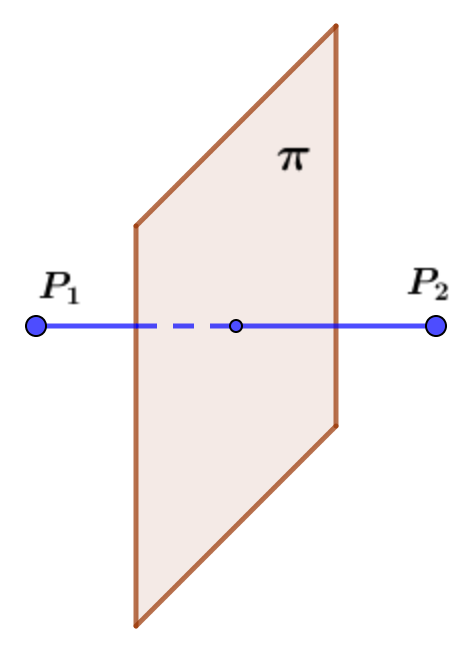
\includegraphics[width=0.2\textwidth]{imagenes/imagenes12/T12IM01.png}
	\end{figure}
	\end{multicols}
	

Decimos que una superficie es simétrica respecto de un plano (llamado plano de simetría) si el simétrico de cada punto de la superficie también es un punto de la superficie.

\begin{itemize}
\item Si la ecuación de una superficie no varía cuando se cambia de signo a dos de sus variables, la superficie es simétrica respecto al eje coordenado de esa variable.
\item Si la ecuación de una superficie no varía cuando se cambia de signo una de sus variables, la superficie es simétrica respecto al plano de la variable que no se cambia.
\item Si la ecuación de una superficie no varía cuando se cambian de signo sus tres variables, la superficie es simétrica respecto del origen de coordenadas.
\end{itemize}


Las pruebas que verifican la simetría de una superficie a partir de su ecuación se muestran en la siguiente tabla:

\begin{table}[H]
\centering
\begin{tabular}{ccc}
\textbf{\begin{tabular}[c]{@{}c@{}}Si $F$ no se altera al \\ cambiar $x$, $y,$ $z$ por:\end{tabular}} & \textbf{$\quad$} & \textbf{\begin{tabular}[c]{@{}c@{}}La superficie es \\ simétrica respecto al:\end{tabular}} \\
$-x,\; y,\; z$    &     & Plano $\;\;YZ$     \\
$x,\; -y,\; z$    &     & Plano $\;\;XZ$     \\
$x,\; y,\; -z$    &     & Plano $\;\;XY$     \\
$-x,\; -y,\; z$    &    & Eje $\;\;Z$     \\
$x,\; -y,\; -z$    &    & Eje $\;\;X$     \\
$-x,\; y,\; -z$    &    & Eje $\;\;Y$     \\
$-x,\; -y,\; -z$    &    & Origen $\;\mathcal O$                                                                                                              
\end{tabular}
\end{table}

\section{Superficie esférica}

Se define la \textbf{\textit{superficie esférica}} como el lugar geométrico de los puntos del espacio que equidistan de un punto fijo. La distancia constante se llama \textbf{radio} y el punto fijo, \textbf{centro}. $\;\boldsymbol{ Esf(C,r) }$

Ecuación de la Esfera (superficie esférica):
$P(x,y,z)\in \mathbb R^3$ es un punto de la esfera de centro $C(a,b,c)$ y radio $r$ $\;\;\left( Esf(C,r) \right)$ si: $\; d(P,C)=r \to \sqrt{(x-a)^2+(y-b)^2+(z-c)^2}=r \to $ Forma ordinaria de la ecuación de la esfera:

\centerline{\colorbox{LightYellow}{$ \boldsymbol{ (x-a)^2+(y-b)^2+(z-c)^2=r^2 } $}} \justify

Desarrollando la ecuación y ordenando los términos tenemos la Forma general de la ecuación de la esfera:

\centerline{\colorbox{LightYellow}{$ \boldsymbol{ x^2+y^2+z^2+Gx+Hy+Iz+K=0 } $}} \justify

Ecuación que contiene cuatro constantes arbitrarias independientes, por lo que una superficie esférica queda unívocamente determinada por cuatro condiciones independientes, por ejemplo,  \underline{cuatro puntos} no coplanarios determinan una \underline{superficie esférica}.

\begin{multicols}{2}
Conviene hacer notar que \textit{el \textbf{plano tangente} a una esfera en cualquiera de sus puntos es \textbf{perpendicular} al \textbf{radio} correspondiente al punto de tangencia.} Es decir, el vector normal al plano tangente $\pi$ a una esfera en uno de sus puntos $\;P\in Esf(C,r)\;$ es $\vec n_{\pi}=\overrightarrow{PC}$.

\begin{figure}[H]
		\centering
		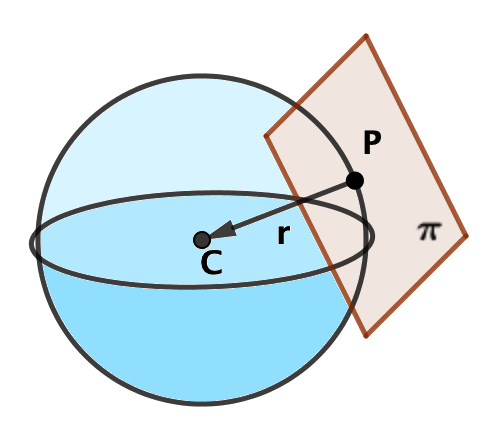
\includegraphics[width=0.4\textwidth]{imagenes/imagenes12/T12IM02.png}
	\end{figure}
\end{multicols}

\begin{ejem}
	Encuentra la ecuación ordinaria y general de la esfera que tiene su centro en $C(0,1,-3)$ y tiene radio $r=4$
\end{ejem}
\noindent $x^2+(y-1)^2+(z+3)^2=4^2\;$ Forma ordinaria, desarrollando:

\noindent $x^2+y^2-2y+1+z^2+6z+9-16=0 \to x^2+y^2+z^2-2y+6z-6=0\;$ Forma general.

\begin{ejem}
Encuentra el centro y el radio de la circunferencia 	dada por $\;x^2+y^2+z^2-2y+6z-6=0$.
\end{ejem}

\noindent Se trata de `completar cuadrados':

\noindent $x^2+y^2+z^2-2y+6z-6=0\to x^2+\textcolor{red}{y^2-2y}\textcolor{blue}{+z^2+6z}-6=0 \to x^2+\textcolor{red}{(y-1)^2-1^2}+\textcolor{blue}{(z+3)^2-3^2-6}=0 \to x^2+(y-1)^2+(z+3)^2-16=0 \to x^2+(y-1)^2+(z+3)^2=4^2 \to \begin{cases} C(0,1,.3) \\ \;\; r=4 \end{cases}$

\begin{ejem}
Encuentra la ecuación de una esfera de centro $C(2,-1,3)$, sabiendo que uno de sus puntos es $P(5,-1,-1)$	
\end{ejem}

\noindent Por definición de esfera, $\; r=d(C,P)=|\overrightarrow{CP}|=\abs{(3,0,-4)}=\sqrt{25}=5$ 

\noindent Luego, la esfera es: $\;(x-2)^2+(y+1)^2+(z-3)^2=5^2$

\begin{ejem}
	Encuentra la ecuación de la esfera que pasa por $P(1,4,3)$, $Q(5,2,3$, $R(6,-1,3)$ y $S(1,-1,8)$
\end{ejem}

\noindent Usaremos la formula general, $Esf\equiv x^2+y*2+z^2+Gx+Hy+Iz+k=0$, donde sustituyendo los puntos $P$, $Q$, $R$, $S$ encontraremos cuatro ecuaciones lineales con cuatro incógnitas:

\noindent $\begin{cases}
P\in Esf \to 1+16+9+E+4F+3G+H=0 \\
Q\in Esf \to 25+4+9+5E+2F+3G+H=0\\
R\in Esf \to 36+1+9+6E-F+3G+H=0 \\
S\in Esf \to 1+1+64+E-F+8G+H=0	
\end{cases}$

\noindent $\left[ \begin{matrix} E&F&G&H \\ 1&4&3&1\\5&2&3&1\\6&-1&3&1\\1&-1&8&1 \end{matrix}\right. \left| \begin{matrix} \\-26\\-38\\-46\\-66\end{matrix}\right] \to $ Resolviendo por Gauss,

\noindent $x^2+y^2+z^2-2x+2y-6z-14=0$, $\;$completando cuadrados:

\noindent $(x-1)^2+(y+1)^2+(z-3)^2=5^2 \to Esf \{  C(1,-1,3);\; r=5 \}$

\begin{ejem}
Encuentra el plano tangente a la esfera $x^2+y^2+z^2=3$ en el  punto $P(1,1,-1)$	
\end{ejem}
\noindent El plano tangente a una esfera es perpendicular al radio en el punto de contacto $P$. Como, evidentemente, el centro de la esfera es $\mathcal O(0,0,0)$, el vector director del plano buscado será: $\; \vec n_{\pi}=\overrightarrow{\mathcal O P}=(1,1,-1)$.

\noindent $\pi: \begin{cases} P(1,1,-1) \\ \vec n_{\pi}=(1,1,-1) \end{cases} \hspace{-3mm} 1(x-1)+1(y-1)-1(z+1)=0\to x+y-z-3=0$


\subsection{Coordenadas esféricas}

Sea $P(x,y,z)$ un punto cualquiera de una superficie esférica de centro en el origen de coordenadas y radio $r$:

$P(x,y,z) \in Esf(\mathcal O, r):\; x^2+t^2+z^2=r^2$

	\begin{figure}[H]
		\centering
		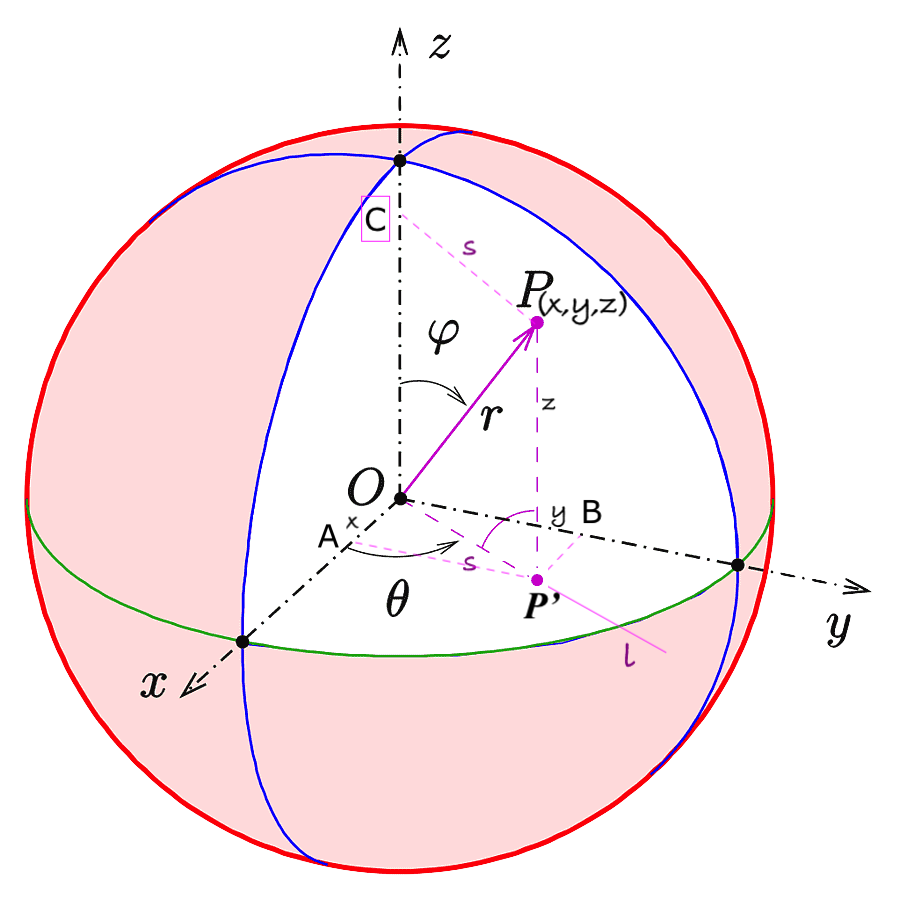
\includegraphics[width=.75\textwidth]{imagenes/imagenes12/T12IM04.png}
	\end{figure}


La porción de esfera comprendida en el primer `octante' aparece el la figura. El punto $P$ y ej eje $OZ$ determinan un plano que corta al plano $XY$ en la recta $l$. 

Llamamos $\theta$ al ángulo formado por $l$ y la parte positiva del eje $OX$ y llamamos $\phi$ al formado por el radio $OP$ y la parte positiva del eje $OZ$. $P',A,B,C$ son, respectivamente, las proyecciones de $P$ sobre $XY$ y sobre los ejes $X,Y,Z$. Sea $\overline{OP'}=\overline{CP}=s$. Del triángulo $OPC$ se tiene que: $\; s=r\sin \phi$.


De los triángulos $OAP'$, $=BP'$ y $=PP'$ se tiene:

\begin{table}[H]
\centering
\begin{tabular}{lll}
$ \boldsymbol{x=s\cos \theta = r \sin \phi \cos \theta} $ \\
$ \boldsymbol{y=s \sin \theta = r \sin \phi \sin \theta} $ \\
$ \boldsymbol{z=\overline{PP'}=r \sin (90^o-\phi)= r \cos \phi} $  
\end{tabular}
\end{table}

De las relaciones $x=r \sin \phi \cos \theta;\; y=r \sin \phi \sin \theta;\; z=r \cos \phi$, es posible localizar cualquier punto $P$ sobre la $Esf(\mathcal O,r)$ conocidos los valores de $r, \theta, \phi$. Estas cantidades, $\boldsymbol{(r, \theta, \phi)}$ se llaman \textbf{coordenadas esféricas}. $\theta$ se llama `longitud', $\phi$ es la `colatitud' y $r$ es el `radio vector' del punto $P(r, \theta, \phi)$. Sus valores están restringidos a los intervalos:
$$r\ge 0;\quad 0\le \pi < \pi;\quad 0\le \theta <2\pi$$

Despejando en las relaciones anteriores, se obtiene:
$$\boldsymbol{ r=\sqrt{x^2+y^2+z^2};\quad \phi=\arccos \dfrac {x}{\sqrt{x^2+y^2+z^2}}; \quad \theta= \arctan
 \dfrac y x }$$
 
 Ecuaciones que, junto a las anteriores, sirven para pasar de coordenadas esféricas $P(r, \phi, \theta)$ a rectangulares $P(x,y,z)$ y viceversa,

\vspace{10mm} % ***************************
\begin{myblock}{Coordenadas Esféricas: resumen}

\begin{table}[H]
\centering
\begin{tabular}{lll}
$ \boldsymbol{x=s\cos \theta = r \sin \phi \cos \theta} $ \\
$ \boldsymbol{y=s \sin \theta = r \sin \phi \sin \theta} $ \\
$ \boldsymbol{z=\overline{PP'}=r \sin (90^o-\phi)= r \cos \phi} $  
\end{tabular}
\end{table}

\vspace{-5mm}$$r\ge 0;\quad 0\le \phi < \pi;\quad 0\le \theta <2\pi$$

\begin{table}[H]
\centering
\begin{tabular}{lll}
$\boldsymbol{ r=\sqrt{x^2+y^2+z^2} }$ \\
$\boldsymbol{ \phi=\arccos \dfrac {x}{\sqrt{x^2+y^2+z^2}} }$ \\
$\boldsymbol{ \theta= \arctan \dfrac y x }$ 
\end{tabular}
\end{table}
\end{myblock}

\section{Superficie cilíndrica}


En general, son ecuaciones del tipo f (x, y) = 0 (análogamente, g(x, z) = 0, h(y,z) = 0); en el plano se corresponden con curvas, en el espacio queda una coordenada libre, luego se corresponden con cilindros, es decir, superficies formadas por rectas que se “levantan” sobre la curva f(x,y) = 0. Los más habituales: 

\begin{itemize}

\item Elípticos: $\dfrac{x^2}{a^2}+\dfrac{y^2}{b^2}=1$. Si $a = b$, se trata de un cilindro circular. 

Si el eje del cilindro está desplazado, pero es paralelo al eje z, se tiene $\dfrac{(x-x_0)^2}{a^2}+\dfrac{(y-y_0)^2}{b^2}=1$. 

Análogamente en $x, z$ ó en  $y, z$. 

\item Parabólicos: $y^2= 2px$. 

Si el eje está desplazado, pero es paralelo al eje z, $(y-y_0)^2=2p(x-x_0)$.  

Análogamente en $x, z$ ó en  $y, z$.
 
\item Hiperbólicos: $\dfrac{x^2}{a^2}-\dfrac{y^2}{b^2}=1$. 

Si el eje del cilindro est á desplazado, pero es paralelo al eje z, se tiene: : $\dfrac{(x-x_0)^2}{a^2}-\dfrac{(y-y_0)^2}{b^2}=1$.
 
Análogamente en $x, z$ ó en  $y, z$. 
\end{itemize}


\begin{figure}[H]
		\centering
		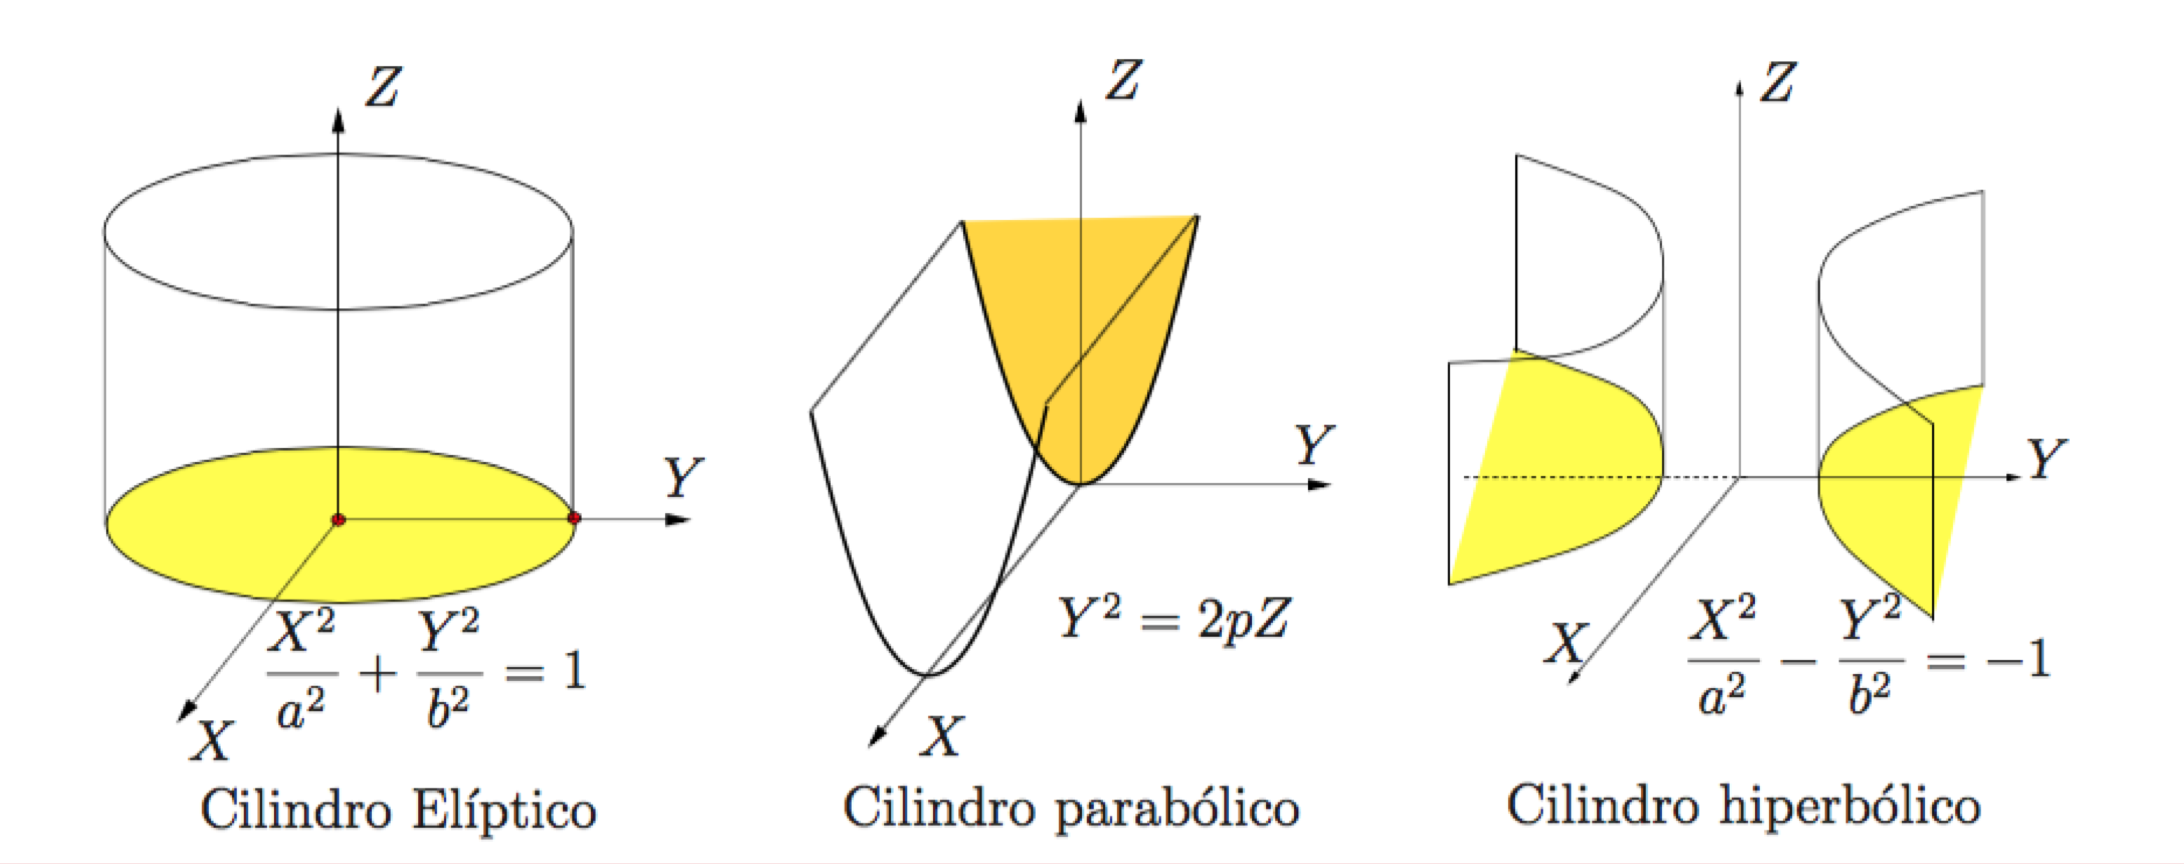
\includegraphics[width=1\textwidth]{imagenes/imagenes12/T12IM05.png}
	\end{figure}

\subsection{Coordenadas cilíndricas}

\begin{figure}[H]
		\centering
		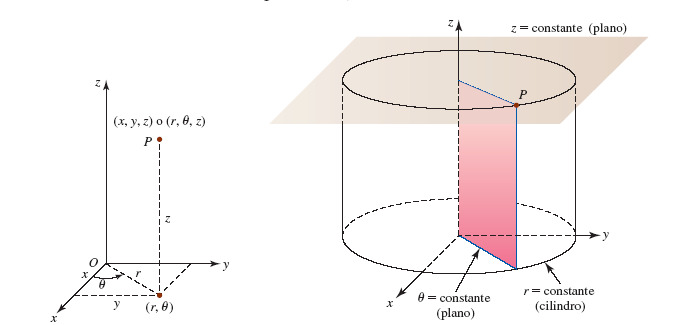
\includegraphics[width=1\textwidth]{imagenes/imagenes12/T12IM06.png}
	\end{figure}

Sea $P(x,y,z)$ un punto cualquiera de la superficie de `un cilindro circular recto' de radio $r$ y cuyo eje es $OZ$. La ecuación de la superficies es $x^2+y^2=r^2;\; forall z$.

Por $P$ y el eje $OZ$ hacemos pasar un plano que corta a la superficie en una generatriz cuya intersección con $XY$ es $P'$. Sea $\overline{PP'}=r$ y llamando $\theta$ al ángulo formado por $OP'$ y la paret positiva del eje $OX$, tenemos:
$$ x=r\cos \theta;\quad y=r \sin \theta;\quad z=z$$

Relaciones que permiten localizar cualquier punto del cilindro conocidos $r,\; \theta,\; z$: $\boldsymbol{P(r,\theta,z)}$ son las \textbf{coordenadas cilíndricas}.

Para que las coordenadas cilíndricas, $r,\; \theta,\; z$, describan un único punto del espacio, adoptamos las siguientes restricciones:
$$ r\ge 0;\quad 0\le \theta < 2 \pi;\quad \forall z \in \mathbb R$$

Despejando estas relaciones, tenemos:
$$r=\sqrt{x^2+y^2}; \quad \theta=\arctan \dfrac y x$$
$$\sin \theta=\dfrac y {\sqrt{x^2+y^2}};\quad x= \dfrac x {\sqrt{x^2+y^2}}$$


 Ecuaciones que, junto a las anteriores, sirven para pasar de coordenadas cilíndricas $P(r, \theta, z)$ a rectangulares $P(x,y,z)$ y viceversa,

\vspace{10mm} % ***************************
\begin{myblock}{Coordenadas Cilíndricas: resumen}
\begin{table}[H]
\centering
\begin{tabular}{lll}
$\boldsymbol{ r\ge 0 }; \qquad  \boldsymbol{ \theta=\arctan \dfrac y x  }; \qquad  \boldsymbol{\forall z}$
\end{tabular}
\end{table}

\vspace{-5mm}$$r\ge 0;\quad 0\le \theta < 2\pi;\quad \forall z$$

\begin{table}[H]
\centering
\begin{tabular}{lll}
$r=\sqrt{x^2+y^2}; \quad \theta=\arctan \dfrac y x$ \\
$\sin \theta=\dfrac y {\sqrt{x^2+y^2}};\quad x= \dfrac x {\sqrt{x^2+y^2}}$ 
\end{tabular}
\end{table}
\end{myblock}


$$ r\ge 0;\quad 0\le \theta < 2 \pi;\quad \forall z \in \mathbb R$$


$$r=\sqrt{x^2+y^2}; \quad \theta=\arctan \dfrac y x$$
$$\sin \theta=\dfrac y {\sqrt{x^2+y^2}};\quad x= \dfrac x {\sqrt{x^2+y^2}}$$


\textit{En el apéndice \ref{VectoresDistintosSistemasCoordenadas} se muestra la forma de expresar el `vector de posición' de un punto en coordenadas cilíndricas y esféricas.}


\section{Superficie cónica}

\begin{multicols}{2}
Es la generada por una recta que se mueve pasando por una curva fija y un punto fijo, no contenido en el plano de esa curva. La recta móvil se llama `generatriz', la curva fija es la `directriz' y el punto fijo es el `vértice' de la cónica, que divide a ésta en dos porciones distintas llamadas `hojas' de la cónica.
	\begin{figure}[H]
		\centering
		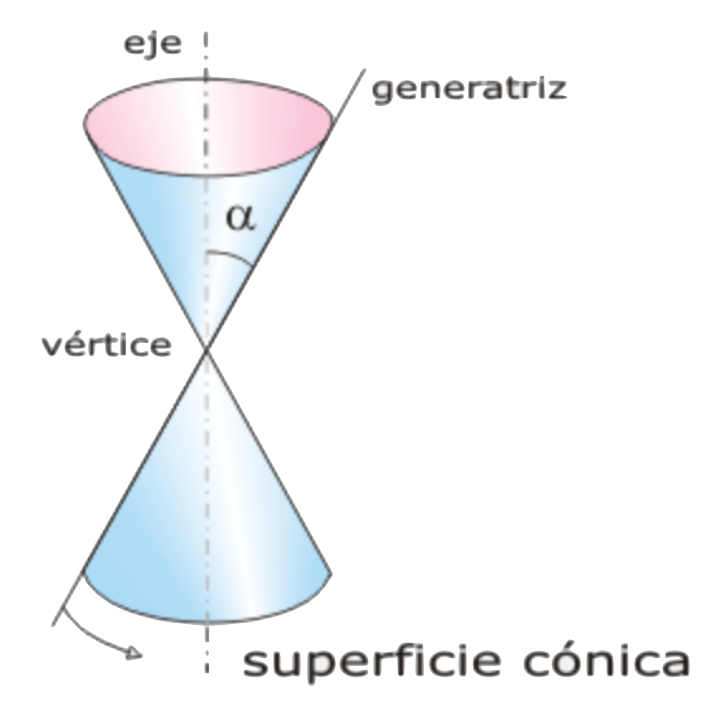
\includegraphics[width=.4\textwidth]{imagenes/imagenes12/T12IM07.png}
	\end{figure}
\end{multicols}


\section{Cuádricas}

Son superficies cuya ecuación es de la forma:

$$ Ax^2+By^2+Cz^2+Dxy+Exz+Fyz+Gx+Hy+Iz+K=0$$,

donde al menos una de las constantes $A, \cdots , F$ es distinta de cero. No todos los posibles valores de las constantes dan lugar a una superficie.

Si una cuádrica se corta por un. plano cualquiera, la curva de intersección es una cónica.

	\begin{figure}[H]
		\centering
		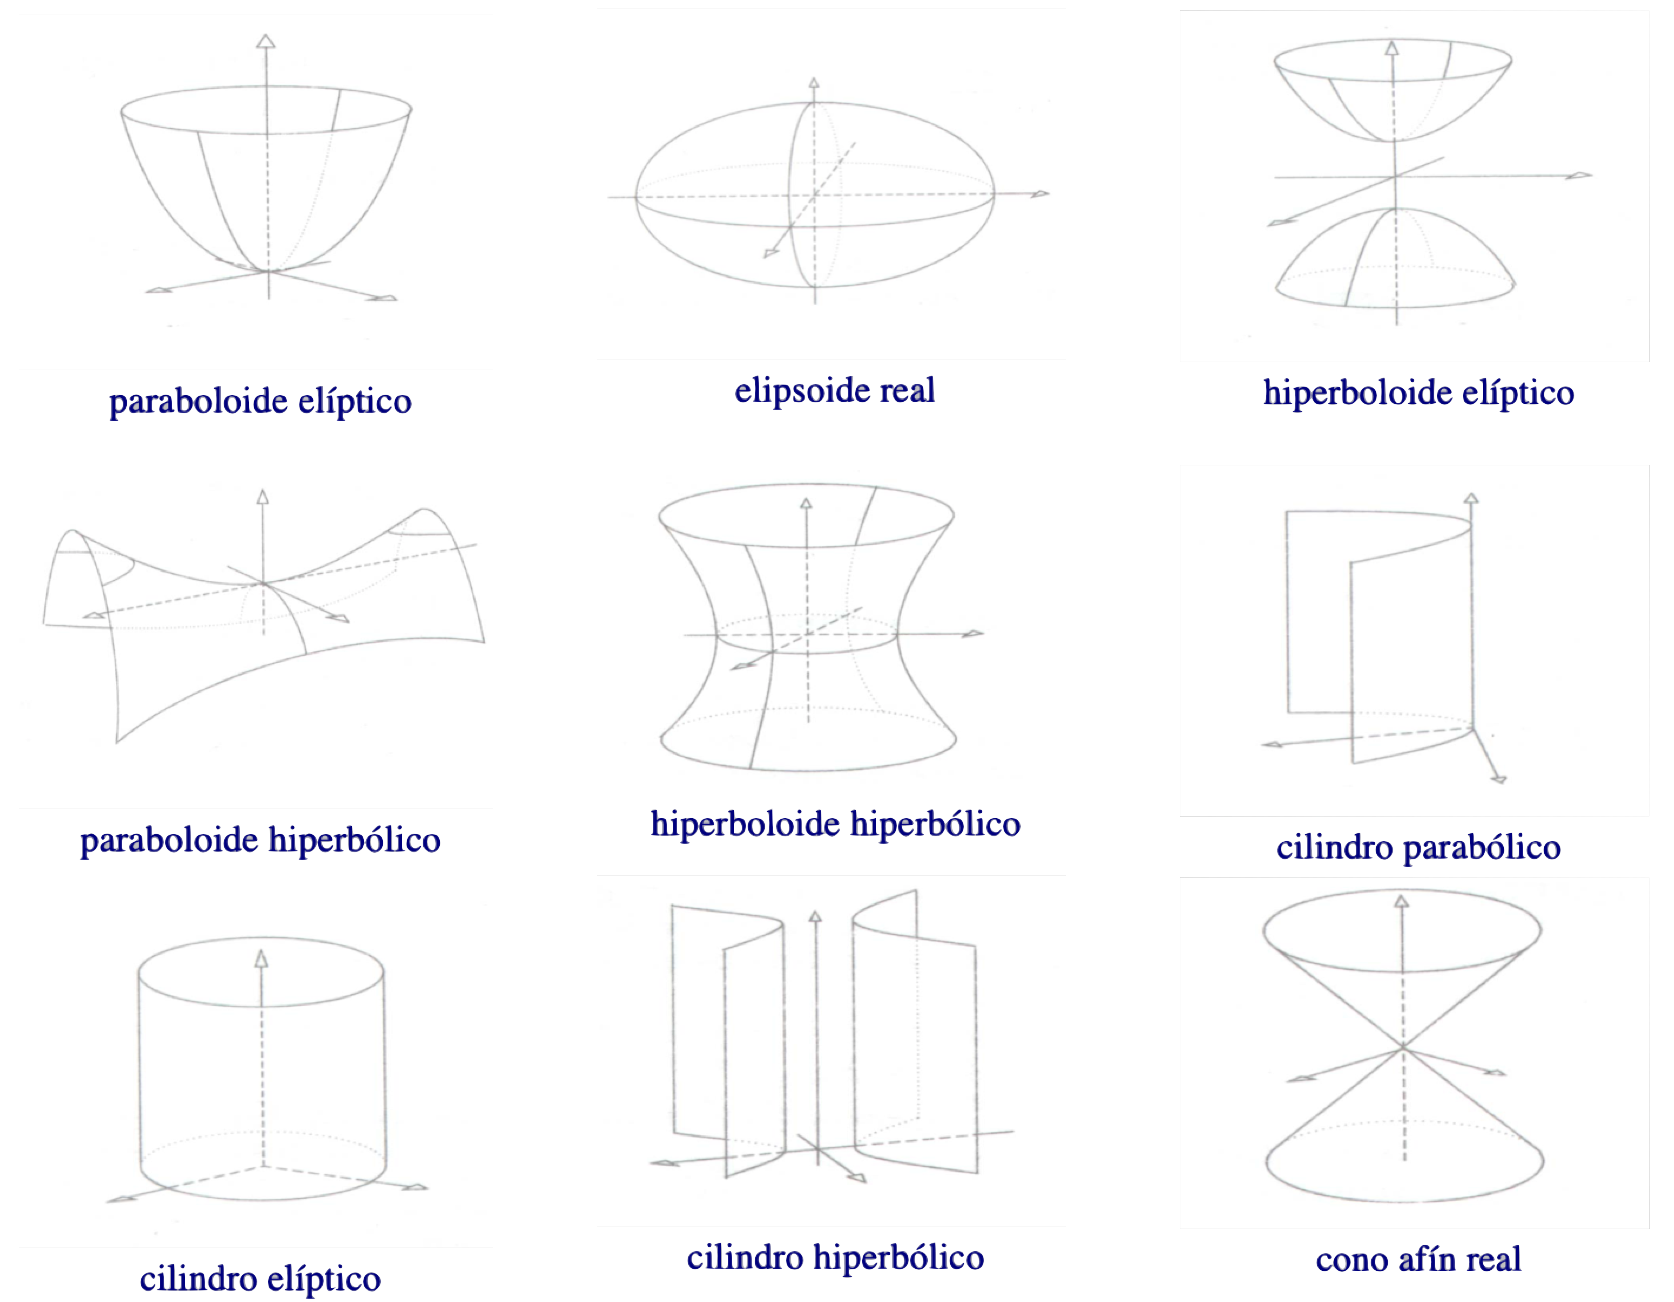
\includegraphics[width=1\textwidth]{imagenes/imagenes12/T12IM08.png}
	\end{figure}


%  \vspace{2mm} \rightline{\textcolor{gris}{\footnotesize{Solución: $1$  }\normalsize{.}}}

%  \rotatebox{180}{\leftline{\textcolor{gris}{tararí}}}.

%  \rotatebox{180}{\leftline{\textcolor{gris}{tararí}}}.

%  \hspace{-10mm}\rotatebox{180}{\leftline{\textcolor{gris}{\footnotesize{ $Resp. 1$  }}}\normalsize{.}}

\begin{comment}
\begin{ejre}
	
\end{ejre}
\begin{proofw}\renewcommand{\qedsymbol}{$\diamond$}	
	
\end{proofw}



	\begin{figure}[H]
		\centering
		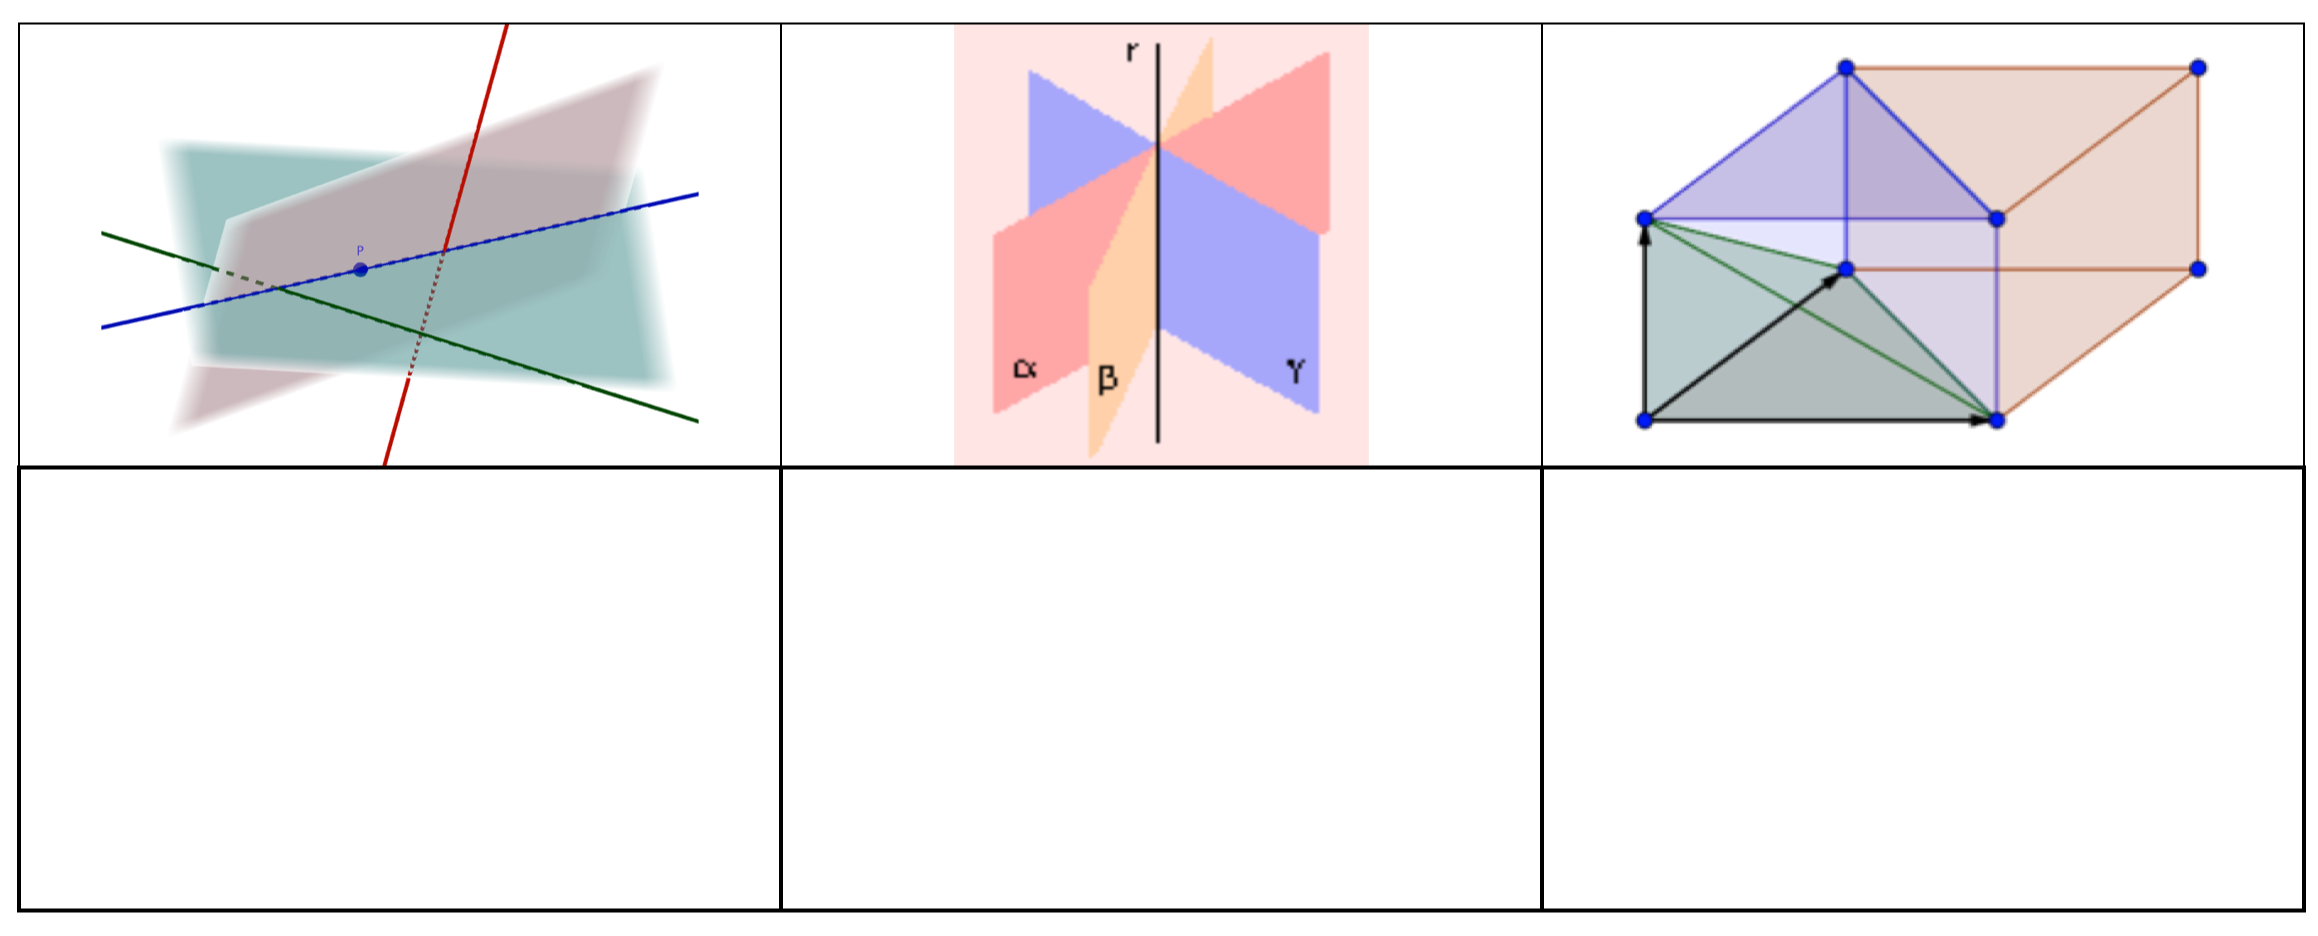
\includegraphics[width=1\textwidth]{imagenes/imagenes11/T11IM38.png}
	\end{figure}

\end{comment}